\documentclass[12pt,a4paper]{article}
\usepackage{amsmath,amssymb,mathrsfs,tikz,times,pifont}
\usepackage{enumitem}
\newcommand\circitem[1]{%
\tikz[baseline=(char.base)]{
\node[circle,draw=gray, fill=red!55,
minimum size=1.2em,inner sep=0] (char) {#1};}}
\newcommand\boxitem[1]{%
\tikz[baseline=(char.base)]{
\node[fill=cyan,
minimum size=1.2em,inner sep=0] (char) {#1};}}
\setlist[enumerate,1]{label=\protect\circitem{\arabic*}}
\setlist[enumerate,2]{label=\protect\boxitem{\alph*}}
%%%::::::by chnini ameur :::::::%%%
\everymath{\displaystyle}
\usepackage[left=1cm,right=1cm,top=1cm,bottom=1.7cm]{geometry}
\usepackage[colorlinks=true, linkcolor=blue, urlcolor=blue, citecolor=blue]{hyperref}
\usepackage{array,multirow}
\usepackage[most]{tcolorbox}
\usepackage{varwidth}
\usepackage{float} %pour utiliser l'option [H] qui force l'image à apparaître exactement à l'endroit où elle est placée dans le code.
\tcbuselibrary{skins,hooks}
\usetikzlibrary{patterns}
%%%::::::by chnini ameur :::::::%%%
\newtcolorbox{exa}[2][]{enhanced,breakable,before skip=2mm,after skip=5mm,
colback=yellow!20!white,colframe=black!20!blue,boxrule=0.5mm,
attach boxed title to top left ={xshift=0.6cm,yshift*=1mm-\tcboxedtitleheight},
fonttitle=\bfseries,
title={#2},#1,
% varwidth boxed title*=-3cm,
boxed title style={frame code={
\path[fill=tcbcolback!30!black]
([yshift=-1mm,xshift=-1mm]frame.north west)
arc[start angle=0,end angle=180,radius=1mm]
([yshift=-1mm,xshift=1mm]frame.north east)
arc[start angle=180,end angle=0,radius=1mm];
\path[left color=tcbcolback!60!black,right color = tcbcolback!60!black,
middle color = tcbcolback!80!black]
([xshift=-2mm]frame.north west) -- ([xshift=2mm]frame.north east)
[rounded corners=1mm]-- ([xshift=1mm,yshift=-1mm]frame.north east)
-- (frame.south east) -- (frame.south west)
-- ([xshift=-1mm,yshift=-1mm]frame.north west)
[sharp corners]-- cycle;
},interior engine=empty,
},interior style={top color=yellow!5}}
%%%%%%%%%%%%%%%%%%%%%%%

\usepackage{fancyhdr}
\usepackage{eso-pic}         % Pour ajouter des éléments en arrière-plan
% Commande pour ajouter du texte en arrière-plan
\usepackage{tkz-tab}
\AddToShipoutPicture{
    \AtTextCenter{%
        \makebox[0pt]{\rotatebox{80}{\textcolor[gray]{0.5}{\fontsize{5cm}{5cm}\selectfont PGB}}}
    }
}
\usepackage{lastpage}
\fancyhf{}
\pagestyle{fancy}
\renewcommand{\footrulewidth}{1pt}
\renewcommand{\headrulewidth}{0pt}
\renewcommand{\footruleskip}{10pt}
\fancyfoot[R]{
\color{blue}\ding{45}\ \textbf{2025}
}
\fancyfoot[L]{
\color{blue}\ding{45}\ \textbf{Prof:M. BA}
}
\cfoot{\bf
\thepage /
\pageref{LastPage}}
\begin{document}
\renewcommand{\arraystretch}{1.5}
\renewcommand{\arrayrulewidth}{1.2pt}
\begin{tikzpicture}[overlay,remember picture]
\node[draw=blue,line width=1.2pt,fill=purple,text=blue,inner sep=3mm,rounded corners,pattern=dots]at ([yshift=-2.5cm]current page.north) {\begingroup\setlength{\fboxsep}{0pt}\colorbox{white}{\begin{tabular}{|*1{>{\centering \arraybackslash}p{0.28\textwidth}} |*2{>{\centering \arraybackslash}p{0.2\textwidth}|} *1{>{\centering \arraybackslash}p{0.19\textwidth}|} }
\hline
\multicolumn{3}{|c|}{$\diamond$$\diamond$$\diamond$\ \textbf{Lycée de Dindéfélo}\ $\diamond$$\diamond$$\diamond$ }& \textbf{A.S. : 2024/2025} \\ \hline
\textbf{Matière: Mathématiques}& \textbf{Niveau : T}\textbf{S2} &\textbf{Date: 28/01/2025} & \textbf{Durée : 4 heures} \\ \hline
\multicolumn{4}{|c|}{\parbox[c]{10cm}{\begin{center}
\textbf{{\Large\sffamily Correction de la composition n$ ^{\circ} $ 1 Du 1$ ^\text{\bf er} $ Semestre}}
\end{center}}} \\ \hline
\end{tabular}}\endgroup};
\end{tikzpicture}
\vspace{3cm}

\section*{\underline{Exercice 1 :} $1,5$ points}

\begin{enumerate}

\item Déterminons les racines cubiques de l'unité.

Résolvons pour cela $z^3 = 1$, $z \in \mathbb{C}$ :

\[
z^3 = 1 \implies z^3 = e^{i(0+2k\pi)}, \quad k \in \mathbb{Z}.
\]

\[
z = e^{i\frac{(0+2k\pi)}{3}}, \quad k = 0, 1, 2.
\]

- Pour $k = 0$, $z = e^{i0} = 1$, donc $z_0 = 1$.

- Pour $k = 1$, $z = e^{i\frac{2\pi}{3}} = \cos\frac{2\pi}{3} + i\sin\frac{2\pi}{3} = -\frac{1}{2} + i\frac{\sqrt{3}}{2}$, donc $z_1 = -\frac{1}{2} + i\frac{\sqrt{3}}{2}$.

- Pour $k = 2$, $z = e^{i\frac{4\pi}{3}} = \cos\frac{4\pi}{3} + i\sin\frac{4\pi}{3} = -\frac{1}{2} - i\frac{\sqrt{3}}{2}$, donc $z_2 = -\frac{1}{2} - i\frac{\sqrt{3}}{2}$.

Ainsi, l'ensemble des solutions est :

\[
.
\]
\[
\tcbhighmath[boxrule=1pt, colback=yellow!5!white, colframe=black]{S_{\mathbb{C}} = \left\{ 1, -\frac{1}{2} + i\frac{\sqrt{3}}{2}, -\frac{1}{2} - i\frac{\sqrt{3}}{2} \right\}
}
\]

\item Interprétation

\begin{itemize}
    \item $\text{arg}(z_B - z_A) = (\overrightarrow{OI}, \overrightarrow{AB}) \, [2\pi]$
    
    Géométriquement, $\text{arg}(z_B - z_A)$ est l'angle $\widehat{(\overrightarrow{OI}, \overrightarrow{AB})}$ formé par le vecteur $\overrightarrow{AB}$ avec l'axe réel du plan complexe $(O, \overrightarrow{OI})$.

    \item $\text{arg}\left(\frac{z_B - z_C}{z_B - z_A}\right) = (\overrightarrow{AB}, \overrightarrow{CD}) \, [2\pi]$
    
    Géométriquement, $\text{arg}\left(\frac{z_B - z_C}{z_B - z_A}\right)$ est l'angle $\widehat{(\overrightarrow{AB}, \overrightarrow{CD})}$ que forment les vecteurs $\overrightarrow{AB}$ et $\overrightarrow{CD}$.
\end{itemize}

\item $f(x) = \sqrt{x}$, appliquons l'IAF

Appliquons l'IAF (Inégalité des Accroissements Finis) sur $[t, t+1]$.

\boxed{
\begin{aligned}
&\textbf{Théorème des Inégalités des Accroissements Finis (TI-AF 1)} \\
&\text{Soit } f \text{ une fonction définie sur un intervalle } [a, b]. \\
&\text{Hypothèses :} \\
&\quad 1) , f \text{ est continue sur } [a, b]. \\
&\quad 2) , f \text{ est dérivable sur } ]a, b[. \\
&\quad 3) , \text{Il existe deux réels } m \text{ et } M \text{ tels que, pour tout } x \in ]a, b[, m \leq f'(x) \leq M. \\
&\text{Conclusion :} \\
&\quad m(b - a) \leq f(b) - f(a) \leq M(b - a). \\
&\textbf{Théorème des Inégalités des Accroissements Finis (TI-AF 2)} \\
&\text{Soit } f \text{ une fonction définie sur un intervalle } [a, b]. \\
&\text{Hypothèses :} \\
&\quad 1) , f \text{ est continue sur } [a, b]. \\
&\quad 2) , f \text{ est dérivable sur } ]a, b[. \\
&\quad 3) , \text{Il existe un réel } m \geq 0 \text{ tel que, pour tout } x \in ]a, b[, |f'(x)| \leq m. \\
&\text{Conclusion :} \\
&\quad |f(b) - f(a)| \leq m|b - a|.
\end{aligned}
}


\textbf{Applications} $t > 0$

\begin{itemize}
    \item $f$ est continue sur $[t, t+1]$.
    \item $f$ est dérivable sur $]t, t+1[$ et pour tout,
\[
    \forall x \in ]t, t+1[, \quad f'(x) = \frac{1}{2\sqrt{x}}.
\]
\end{itemize}

Comme $x \in ]t, t+1[$, alors $t < x < t+1$. Ainsi, 
\[
\frac{1}{2\sqrt{t+1}} < \frac{1}{2\sqrt{x}} < \frac{1}{2\sqrt{t}}.
\]

D'où :
\[
\frac{1}{2\sqrt{t+1}} < f'(x) < \frac{1}{2\sqrt{t}}.
\]

En appliquant l'inégalité des accroissements finis (IAF), nous avons :
\[
\frac{1}{2\sqrt{t+1}}(t+1-t) < f(t+1) - f(t) < \frac{1}{2\sqrt{t}}(t+1-t).
\]

Cela donne :
\[
\frac{1}{2\sqrt{t+1}} < f(t+1) - f(t) < \frac{1}{2\sqrt{t}}.
\]

\end{enumerate}

\section*{\underline{Exercice 2 :} 8,5 points}

\subsection*{ Partie A}
\begin{enumerate}
\item Montrons que $P$ admet une unique racine réelle.

Soit $z_0 = a \in \mathbb{R}$ tel que $P(z_0) = 0$.

\[
P(z) = z^3 + (-5 + 2i)z^2 + (7 - 7i)z - 2 + 6i
\]

\[
P(z_0) = 0 \implies a^3 + (-5 + 2i)a^2 + (7 - 7i)a - 2 + 6i = 0
\]

\[
\implies a^3 - 5a^2 + 7a - 2 + i\big(2a^2 - 7a + 6\big) = 0
\]

En séparant les parties réelle et imaginaire :
\[
\begin{cases}
a^3 - 5a^2 + 7a - 2 = 0 \quad (1) \\
2a^2 - 7a + 6 = 0 \quad (2)
\end{cases}
\]

L'équation (2) est plus facile à résoudre.

Résolution de (2)

\[
2a^2 - 7a + 6 = 0
\]

Calculons le discriminant :
\[
\Delta = 7^2 - 4 \times 2 \times 6 = 49 - 48 = 1.
\]

Les solutions sont :
\[
a_1 = \frac{-(-7) - \sqrt{\Delta}}{2 \times 2} = \frac{7 - 1}{4} = \frac{6}{4} = \frac{3}{2},
\]
\[
a_2 = \frac{-(-7) + \sqrt{\Delta}}{2 \times 2} = \frac{7 + 1}{4} = \frac{8}{4} = 2.
\]

La racine de (2) qui vérifie (1) est la racine de $P(z)$.

Vérification pour $a = \frac{3}{2}$

\underline{Substituons $a = \frac{3}{2}$ dans (1) :}
\begin{align*}
a^3 - 5a^2 + 7a - 2 &= \left(\frac{3}{2}\right)^3 - 5\left(\frac{3}{2}\right)^2 + 7\left(\frac{3}{2}\right) - 2\\
										&=\frac{27}{8} - 5 \times \frac{9}{4} + \frac{21}{2} - 2\\
										&=\frac{27}{8} - \frac{45}{8} + \frac{84}{8} - \frac{16}{8}\\
										&=\frac{27 - 45 + 84 - 16}{8}\\
										&= \frac{111 - 106}{8} = \frac{5}{8} \neq 0
\end{align*}

Donc, $a = \frac{3}{2}$ n'est pas solution.

\underline{Vérification pour $a = 2$}

Substituons $a = 2$ dans (1) :

\begin{align*}
a^3 - 5a^2 + 7a - 2 &= 2^3 - 5(2^2) + 7(2) - 2\\
										&=8 - 20 + 14 - 2\\
										&=0
\end{align*}

Donc, $a = 2$ est une solution.

\[
\tcbhighmath[boxrule=1pt, colback=yellow!5!white, colframe=black]{ z_0 = 2. }
\]
\item Factorisons $P(z)$

Utilisons la méthode de la division synthétique pour factoriser $P(z)$. Le tableau est donné ci-dessous :

\[
\begin{array}{|c|c|c|c|c|}
\hline
\text{ } & 1 & -5+2i & 7-7i & 2+6i \\ 
\hline
2 & \downarrow & 2 & -6+i & 2-6i \\ 
\hline
\text{ } & 1 & -3+2i & 1-3i & 0 \\ 
\hline
\end{array}
\]

Ainsi, nous avons :

\[
\tcbhighmath[boxrule=1pt, colback=yellow!5!white, colframe=black]{ P(z) = (z - 2)\big(z^2 + (-3+2i)z + 1-3i\big) }
\]
\item Résolvons $P(z) = 0$

\[
P(z) = 0 \implies z = 2 \quad \text{ou} \quad z^2 + (-3+2i)z + 1-3i = 0.
\]

\begin{align*}
\Delta &= (-3+2i)^2 - 4(1)(1-3i)\\
 			 &= 9 - 12i - 4 + 12i\\
	     &= 5
\end{align*}

\[
z_{1} = \frac{3-\sqrt{5}}{2}-i, z_{2} = \frac{3+\sqrt{5}}{2}-i
\]

\[
\tcbhighmath[boxrule=1pt, colback=yellow!5!white, colframe=black]{ S = \left\{ 2, \frac{3-\sqrt{5}}{2}-i, \frac{3+\sqrt{5}}{2}-i \right\} }
\]
\end{enumerate}
\subsection*{ Partie B}

\begin{enumerate}
\item Représentation

\begin{center}
\begin{tikzpicture}[scale=2]

    % Axes avec origine décalée à gauche
    \draw[->] (-1,0) -- (3.5,0) node[below] {\( \text{Re} \)};
    \draw[->] (0,-1.5) -- (0,2.5) node[left] {\( \text{Im} \)};
    
    % Cercle unité pour illustration de l'angle
    \draw[dashed, gray] (0,0) circle(1);

    % Points
    \filldraw[red] (2,-1) circle(2pt) node[below right] {\( A(2,-1) \)};
    \filldraw[red] (2,0) circle(2pt) node[above right] {\( B(2) \)};
    \filldraw[red] (1,-1) circle(2pt) node[below left] {\( C(1,-1) \)};
    \filldraw[red] (1,0) circle(2pt) node[above left] {\( D(1) \)};
    
    % Lignes de connexion
    \draw[thick, dashed, blue] (2,-1) -- (2,0) -- (1,0) -- (1,-1) -- cycle;
    
    % Angle de π/3
    \draw[thick] (0.7,0) arc[start angle=0, end angle=60, radius=0.7];
    \node at (0.9,0.3) {\(\frac{\pi}{3}\)};
    
    % Vecteur illustrant un nombre complexe sur le cercle
    \draw[thick, ->] (0,0) -- (cos{60},sin{60});
    
\end{tikzpicture}
\end{center}

\item Écriture exponentielle de $z_C$ et $z_E$

\underline{Pour $z_C$ :}

\begin{align*}
z_C &= 1 - i\\
		&= \sqrt{2} \left(\cos\left(-\frac{\pi}{4}\right) + i\sin\left(-\frac{\pi}{4}\right)\right)\\
		&= \sqrt{2} e^{-i\frac{\pi}{4}}\\
\end{align*}

\[
\tcbhighmath[boxrule=1pt, colback=yellow!5!white, colframe=black]{ z_C=\sqrt{2} e^{-i\frac{\pi}{4}} }
\]
\underline{Pour $z_E$ :}

\begin{align*}
z_E &= 1 + i\sqrt{3}\\
	  &= 2 \left(\frac{1}{2} + i\frac{\sqrt{3}}{2}\right)\\
		&= 2 \left(\cos\left(\frac{\pi}{3}\right) + i\sin\left(\frac{\pi}{3}\right)\right)\\
		&= 2 e^{i\frac{\pi}{3}}
\end{align*}

Donc :

\[
\tcbhighmath[boxrule=1pt, colback=yellow!5!white, colframe=black]{ z_E = 2 e^{i\frac{\pi}{3} }}
\]
\item Plaçons exactement le point $E$

\[
z_E = 2 e^{i\pi/3}.
\]

\item Écriture algébrique de $z_E^8$

\begin{align*}
z_E = 2 e^{i\pi/3} &\implies z_E^8 = 2^8 e^{8i\pi/3}\\
                   &\implies z_E^8=2^8 \left[\cos\left(\frac{2\times 3\pi}{3}+\frac{2\pi}{3}\right) + i\sin\left(\frac{2\times 3\pi}{3}+\frac{2\pi}{3}\right)\right]\\
										&\implies z_E^8=\left[\cos\left(2\pi+\frac{2\pi}{3}\right) + i\sin\left(2\pi+\frac{2\pi}{3}\right)\right]\\
										&\implies z_E^8 = 2^8 \left(-\frac{1}{2} + i\frac{\sqrt{3}}{2}\right)
\end{align*}

\[
\tcbhighmath[boxrule=1pt, colback=yellow!5!white, colframe=black]{ zz_E^8 = 2^8 \left(-\frac{1}{2} + i\frac{\sqrt{3}}{2}\right) }
\]
\item Calculons les affixes de $I$ et $J$

On a : $ I = \text{bar}\{(A,1); (C,-2)\} $
\begin{align*}
I = \text{bar}\{(A,1); (C,-2)\} &\implies \overrightarrow{AI} = \frac{-2}{1-2} \overrightarrow{AC}\\
                                &\implies \overrightarrow{AI} = 2 \overrightarrow{AC}\\
                                &\implies Z_I - Z_A = 2 (Z_C - Z_A)\\
                                &\implies Z_I - Z_A = 2Z_C - 2Z_A\\
                                &\implies Z_I = 2Z_C - Z_A\\
                                &\implies Z_I = 2 (1 - i) - (2 - i)\\
                                &\implies Z_I = 2 - 2i - 2 + i\\
                                &\implies Z_I = -i.
\end{align*}

\[
\tcbhighmath[boxrule=1pt, colback=yellow!5!white, colframe=black]{ Z_I = -i }
\]


On a: $ J = \text{bar}\{(A,1); (C,2)\} $

\begin{align*}
\text{Donc } J = \text{bar}\{(A,1); (C,2)\} &\implies \overrightarrow{AJ} = \frac{2}{1+2} \overrightarrow{AC}\\
															 &\implies Z_J - Z_A = \frac{2}{3} Z_C - \frac{2}{3} Z_A\\
                               &\implies Z_J = \frac{2}{3} Z_C + \frac{1}{3} Z_A\\
                               &\implies Z_J = \frac{2}{3} (1 - i) + \frac{1}{3} (2 - i)\\
                               &\implies Z_J = \frac{2}{3} + \frac{2}{3} (-i) + \frac{2}{3} - \frac{i}{3}\\
                               &\implies Z_J = \frac{4}{3} - i
\end{align*}

\[
\tcbhighmath[boxrule=1pt, colback=yellow!5!white, colframe=black]{ Z_J = \frac{4}{3} - i }
\]
\item Donner un module et un argument de $\frac{Z_B - Z_A}{Z_C - Z_A}$

\begin{align*}
\frac{Z_B - Z_A}{Z_C - Z_A} &= \frac{2 - (2 - i)}{1 - i - (2 - i)}\\
														&= \frac{i}{-1}\\
														&= i
\end{align*}

\[
\tcbhighmath[boxrule=1pt, colback=yellow!5!white, colframe=black]{ \frac{Z_B - Z_A}{Z_C - Z_A} = i }
\]
\textbf{Module}

\[
\left| \frac{Z_B - Z_A}{Z_C - Z_A} \right| = |i| = 1
\]
\[
\tcbhighmath[boxrule=1pt, colback=yellow!5!white, colframe=black]{ \left| \frac{Z_B - Z_A}{Z_C - Z_A} \right| = |i| = 1 }
\]
\textbf{Un Argument}

\[
\arg\left( \frac{Z_B - Z_A}{Z_C - Z_A} \right) = \frac{\pi}{2}
\]
\[
\tcbhighmath[boxrule=1pt, colback=yellow!5!white, colframe=black]{ \arg\left( \frac{Z_B - Z_A}{Z_C - Z_A} \right) = \frac{\pi}{2} }
\]
\item Nature de $ABC$

\[
\begin{cases}
\left| \frac{Z_B - Z_A}{Z_C - Z_A} \right| = 1\\
\arg\left( \frac{Z_B - Z_A}{Z_C - Z_A} \right) = \frac{\pi}{2} 
\end{cases}\implies
\begin{cases}
AB = AC\\
\left(\overrightarrow{AC},\overrightarrow{AB} \right) = \frac{\pi}{2}
\end{cases}
\]
%\left( \widehat{ACB}, \widehat{CAB} \right) = \frac{\pi}{2}
\[
\text{Donc } ABC \text{ est un triangle rectangle et isocèle en } A.
\]

\item Montrons que $A, B, C, D$ sont cocycliques

On a :

\[
BD = |Z_D - Z_B| = |1 - 2| = 1
\]

\[
DC = |Z_C - Z_D| = |i - i - 1| = 1
\]

\textbf{Conclusion} 

\[
\text{donc } AB = AC = BD = DC \quad \text{et} \quad \widehat{(AC, AB)} = \frac{\pi}{2}.
\]

\[
\text{donc } ABDC \text{ est un carré, donc il est inscrit dans un cercle } \mathcal{C}\left(\frac{z_{A}+z_{D}}{2},\frac{|z_{A}-z_{D}|}{2} \right) .
\]

\[
\text{Tel que les sommets de } ABCD \text{ appartiennent à } \mathcal{C}.
\]

\begin{align*}
\frac{z_{A}+z_{D}}{2}&=\frac{2-i+1}{2}\\
					 &=\frac{3-i}{2}\\
\end{align*}

\begin{align*}
\frac{|z_{A}-z_{D}|}{2}&=\frac{|2-i-1|}{2}\\
						&=\frac{|1-i|}{2}\\
						&=\frac{\sqrt{2}}{2}
\end{align*}

\[
\tcbhighmath[boxrule=1pt, colback=yellow!5!white, colframe=black]{ \mathcal{C}\left( \left( \frac{3-i}{2} \right) , \frac{\sqrt{2}}{2} \right) }
\]

\[
\tcbhighmath[boxrule=1pt, colback=yellow!5!white, colframe=black]{ \mathcal{C} \left( \begin{pmatrix} \frac{3}{2} \\ -\frac{1}{2} \end{pmatrix}, \frac{\sqrt{2}}{2} \right) }
\]
\item Forme exponentielle de $Z$ et Écriture algébrique $Z$

\begin{enumerate}
\item Forme exponentielle de $Z$
\[
Z = \frac{Z_E}{Z_C}
\]


\begin{align*}
\begin{cases}
Z_E = 2 e^{i\pi/3}\\
Z_C = \sqrt{2} e^{-i\pi/4}
\end{cases}
&\iff Z = \frac{2 e^{i\pi/3}}{\sqrt{2} e^{-i\pi/4}}\\
&\iff Z = \sqrt{2} e^{i(\pi/3 + \pi/4)}\\
&\iff Z = \sqrt{2} e^{i\frac{7\pi}{12}}
\end{align*}

\[
\tcbhighmath[boxrule=1pt, colback=yellow!5!white, colframe=black]{ Z = \sqrt{2} e^{i\frac{7\pi}{12}} }
\]
\item Les valeurs de $\cos\frac{7\pi}{12}$ et $\sin\frac{7\pi}{12}$

Écriture algébrique de $Z$
\begin{align*}
Z = \frac{Z_E}{Z_C}\iff Z &= \frac{1 + i\sqrt{3}}{1 - i}\\
  &= \frac{(1 + i\sqrt{3})(1 + i)}{(1 - i)(1 + i)}\\
 &= \frac{(1 + i\sqrt{3})(1 + i)}{2}\\
 &= \frac{1 + \sqrt{3}i + i - \sqrt{3}}{2}\\
Z &= \frac{1 - \sqrt{3}}{2} + i \frac{1 + \sqrt{3}}{2}
\end{align*}

\begin{align*}
Z &= \sqrt{2} e^{i\frac{7\pi}{12}}\\
Z &= \sqrt{2} \left[\cos\left(\frac{7\pi}{12}\right) + i\sin\left(\frac{7\pi}{12}\right)\right].
\end{align*}

\[
\text{Par identification : }\cos\left(\frac{7\pi}{12}\right) = \frac{\frac{1 - \sqrt{3}}{2}}{\sqrt{2}}, \quad \sin\left(\frac{7\pi}{12}\right) = \frac{\frac{1 + \sqrt{3}}{2}}{\sqrt{2}}.
\]

\[ \text{D'où : }
\tcbhighmath[boxrule=1pt, colback=yellow!5!white, colframe=black]{ \cos\left(\frac{7\pi}{12}\right) = \frac{\sqrt{2} - \sqrt{6}}{4}, \quad \sin\left(\frac{7\pi}{12}\right) = \frac{\sqrt{2} + \sqrt{6}}{4} }
\]
\end{enumerate}

\end{enumerate}
\subsection*{ Partie C}

Soit $f$ définie par :
$$
\begin{array}{rcl}
f : \mathbb{P} \setminus \{c(1 - i)\}&\to& \mathbb{P}\\
Z &\mapsto &\frac{Z - 2i}{Z - 1 + i}
\end{array}
$$
\begin{enumerate}
\item Expression de $OM'$ en fonction de $MA$ et $MC$
On a :
\[
Z' = \frac{Z - 2i}{Z - 1 + i}.
\]

\[
Z' = \frac{Z - (2 + i)}{Z - (1 + i)}.
\]

\[
Z' = \frac{Z_M - Z_A}{Z_M - Z_C}.
\]

\[
|Z'_M| = \left|\frac{Z_M - Z_A}{Z_M - Z_C}\right|.
\]

\[
OM' = \frac{MA}{MC}.
\]

\[
\tcbhighmath[boxrule=1pt, colback=yellow!5!white, colframe=black]{ OM' = \frac{MA}{MC} }
\]
\item Une interprétation géométrique de $\arg(Z')$

$\arg(Z')=\arg\left( \frac{Z_M - Z_A}{Z_M - Z_C} \right) = \left( \overrightarrow{CM};\overrightarrow{AM} \right) = \left( \overrightarrow{MC};\overrightarrow{MA} \right) $

Géométriquement, $\arg(Z')$ représente l'angle orienté entre les vecteurs $\overrightarrow{CM}$ et $\overrightarrow{AM}$.
\item L'ensemble des points M pour $Z'$ soit un réel non nul.
 \[
    Z' = \frac{Z_M - Z_A}{Z_M - Z_C}.
    \]

    Pour que $Z'$ soit un réel non nul, deux conditions doivent être satisfaites :
    \begin{enumerate}
        \item \( Z_M \neq Z_A \), car le numérateur ne doit pas être nul.
        \item \( Z_M \neq Z_C \), car le dénominateur ne doit pas être nul.
    \end{enumerate}

    Ensuite, pour que \( Z' \) soit un réel, l'argument de \(\frac{Z_M - Z_A}{Z_M - Z_C}\) doit être nul ou un multiple de \(\pi\),\\$\arg(Z')=\arg\left( \frac{Z_M - Z_A}{Z_M - Z_C} \right)=0[\pi]$, ce qui implique que les vecteurs \(\overrightarrow{CM}\) et \(\overrightarrow{AM}\) sont colinéaires.

    En termes géométriques, cela signifie que \( M \) appartient à la droite passant par \( A \) et \( C \), à l'exclusion des points \( A \) et \( C \).

    L'ensemble des points \( M \) est donc donné par :
    \[
    \mathcal{D} = \{M \in \mathbb{C} \mid M \in \text{droite}(A, C) \setminus \{A, C\}\}.
    \]
\item Donner et construire l'ensemble des points M tel que \( |Z'|=2 \)
\[
|Z'_M| = \left|\frac{Z_M - Z_A}{Z_M - Z_C}\right|=OM = \frac{MA}{MC}.
\]

\begin{align*}
MA =2MC &\implies (MA)^{2} =(2MC)^{2}\\
				&\implies (MA)^{2} -(2MC)^{2}=0\\
				&\implies (\overrightarrow{MA} - 2\overrightarrow{MC}).(\overrightarrow{MA} + 2\overrightarrow{MC}) = 0\\
\text{Or }  I = \text{bar}\{(A,1); (C,-2)\} \text{ et } J = \text{bar}\{(A,1); (C,2)\}\\
				&\implies (1-2)\overrightarrow{MI}.(2+1)\overrightarrow{MJ} = 0\\
				&\implies -3\overrightarrow{MI}.\overrightarrow{MJ} = 0\\
				&\implies \overrightarrow{MI}.\overrightarrow{MJ} = 0
\end{align*}

\( M \) décrit donc un cercle de centre $\frac{z_I+z_J}{2}$ et de rayon $\frac{|z_I-z_J|}{2}$

$ \frac{z_I+z_J}{2} = \frac{ -i+\left( \frac{4}{3} - i\right) }{2} $ \text{ et } $\frac{|z_I-z_J|}{2}=\frac{|-i-\left( \frac{4}{3} - i\right)|}{2} $

$ \frac{z_I+z_J}{2} = \frac{ \left( \frac{4}{3} - 2i\right) }{2} $ \text{ et } $\frac{|z_I-z_J|}{2}=\frac{|-\frac{4}{3}|}{2} $

$ \frac{z_I+z_J}{2} = \frac{ \left( \frac{4 - 6i}{3}\right) }{2} $ \text{ et } $\frac{|z_I-z_J|}{2}=\frac{4}{6} $

$ \frac{z_I+z_J}{2} = \frac{4 - 6i}{6} $ \text{ et } $\frac{|z_I-z_J|}{2}=\frac{4}{6} $

$ \frac{z_I+z_J}{2} = \frac{2 - 3i}{3} $ \text{ et } $\frac{|z_I-z_J|}{2}=\frac{4}{6} $

$ \frac{z_I+z_J}{2} = \frac{2}{3}-i $ \text{ et } $\frac{|z_I-z_J|}{2}=\frac{4}{6} $

\[ \text{Finalement : } 
\tcbhighmath[boxrule=1pt, colback=yellow!5!white, colframe=black]{ \mathcal{C}\left( \left( \frac{2}{3}-i \right)  ;\frac{4}{6}\right) }
\]

\[
\tcbhighmath[boxrule=1pt, colback=yellow!5!white, colframe=black]{ \mathcal{C} \left( \begin{pmatrix} \frac{3}{2} \\ -1 \end{pmatrix}, \frac{4}{6} \right) }
\]
\end{enumerate}

\section*{\underline{Problème :} 10 points}

\subsection*{Partie A}

\begin{enumerate}

\item
\begin{enumerate}
    \item Montrons que \( \forall x > -3, \; u(x) = 2 - \frac{2}{x+3} \).
    
    \[
    \text{On a } u(x) = \frac{2x+1}{x+3}
    \]

    \begin{align*}
        u(x) &= \frac{2x + 6 - 2}{x+3} \\
        &= \frac{2(x+3) - 2}{x+3} \\
        &= 2 - \frac{2}{x+3}
    \end{align*}

    \item Limites de \( u \) aux bornes de \( ]-3, +\infty[ \) :

    \textbf{En \( -3^+ \)} :
    
    \begin{align*}
    \lim_{x \to -3^+} u(x) &= \lim_{x \to -3^+} \left( 2 - \frac{2}{x+3} \right) \\
    &= 2 - \lim_{x \to -3^+} \frac{2}{x+3} \\
    &= 2 - \frac{2}{0^+} \\
    &= 2 - (+\infty) \\
    &= +\infty
    \end{align*}

    \[
    \text{Donc } \lim_{x \to -3^+} u(x) = +\infty
    \]

    \textbf{En \( +\infty \)} :
    
    \begin{align*}
    \lim_{x \to +\infty} u(x) &= \lim_{x \to +\infty} \left( 2 - \frac{2}{x+3} \right) \\
    &= 2 - \lim_{x \to +\infty} \frac{2}{x+3} \\
    &= 2 - 0 \\
    &= 2
    \end{align*}

    \[
    \text{Donc } \lim_{x \to +\infty} u(x) = 2
    \]

    \item \textbf{La primitive \( G \) de \( u \) telle que \( G(-2) = 0 \)} :
    
    \[
    u(x) = 2 - \frac{2}{x+3} \quad \text{donc} \quad G(x) = 2x - 2\ln(x+3) + k, \; \text{avec } k \in \mathbb{R}.
    \]

    \begin{align*}
    G(-2) &= 2(-2) - 2\ln(-2+3) + k \\
    &= -4 - 2\ln(1) + k \\
    &= -4 + k.
    \end{align*}

       Or \( G(-2) = 0 \) :
    \[
    -4 + k = 0 \quad \implies \quad k = 4.
    \]

    Donc :
    \[
    G(x) = 2x - 2\ln(x+3) + 4.
    \]
\end{enumerate}

\item
\begin{enumerate}
    \item \textbf{Calcul de \( u(-2) \)} :

    \[
    u(-2) = 2 - \frac{2}{-2+3} \implies u(-2) = 2 - 2 \implies u(-2) = 0.
    \]

    \[
    \text{Donc } u(-2) = 0.
    \]
    
    \textbf{Tableau de variation de \( G \)}

\( G \) est la primitive de \( u \) sur \( ]-3, +\infty[ \), donc :$ G'(x) = u(x), \; \forall x \in ]-3, +\infty[. $

Étude du signe de \( u(x) \) sur \( ]-3, +\infty[ \) :

\begin{center}

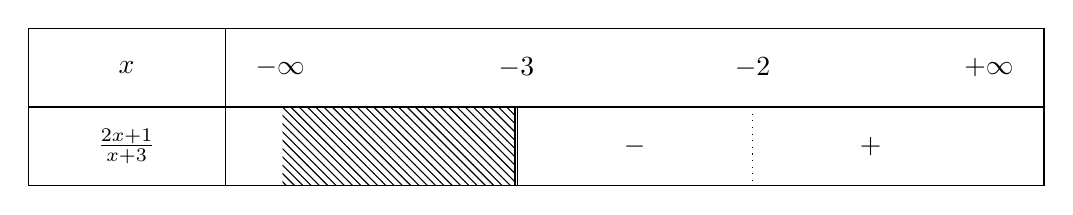
\begin{tikzpicture}
   \tkzTabInit[lgt = 2.5, espcl = 3, deltacl = 0.7]{$x$ / 1 , $\frac{2x+1}{x+3}$ / 1 }{$-\infty$, $-3$, $-2$, $+\infty$}
   \tkzTabLine{,h, d, - ,t, +, }
\end{tikzpicture}

\end{center}

- \( \forall x \in ]-3, -2[, u(x) < 0 \) donc \( G \) est décroissante.

- \( \forall x \in ]-2, +\infty[, u(x) > 0 \) donc \( G \) est croissante.

\textbf{Limites aux bornes de \( D_G = ]-3, +\infty[ \) :}

\textbf{En \( -3^+ \) :}

\begin{align*}
\lim_{x \to -3^+} G(x) &= \lim_{x \to -3^+} \left( 2x - 2\ln(x+3) + 4 \right) \\
&= 2(-3) - 2\ln(0^+) + 4 \\
&= -6 - 2(-\infty) + 4 \\
&= +\infty
\end{align*}

\[
\text{Donc } \lim_{x \to -3^+} G(x) = +\infty
\]

\textbf{En \( +\infty \) :}

\begin{align*}
\lim_{x \to +\infty} G(x) &= \lim_{x \to +\infty} \left( 2x - 2\ln(x+3) + 4 \right) \\
&= \lim_{x \to +\infty} \frac{2x}{x+3} - \lim_{x \to +\infty} \frac{2\ln(x+3)}{x+3} + \lim_{x \to +\infty} \frac{4}{x+3} \\
&= 2 - 0 + 0 \\
&= 2
\end{align*}

\[
\text{Donc } \lim_{x \to +\infty} G(x) = 2
\]

\begin{center}
    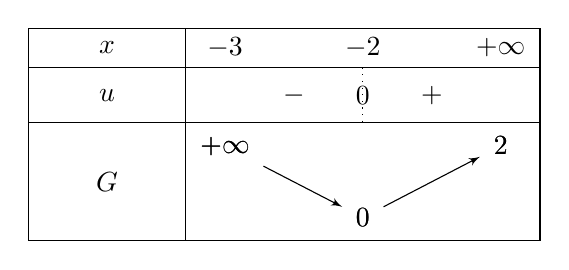
\begin{tikzpicture}[node style/.style={fill opacity=0,text opacity=1}]
        \tkzTabInit[espcl=1.75]{$x$/.5,$u$/.7,$G$/1.5}{$-3$,$-2$,$+\infty$}
        \tkzTabLine{,-,z,+,}
        \tkzTabVar{+/$+\infty$, -/$0$, +/$2$} 
    \end{tikzpicture}
\end{center}

\end{enumerate}
\item  Le signe de G.

\(\forall x \in ]-3;+\infty[\)
\end{enumerate}

\subsection*{Partie B}

\[
f(x) =
\begin{cases}
\sqrt{x^2 + 2x} & \text{si } x \leq -2, \\
\ln\left(\frac{2x + 1}{x + 3}\right) & \text{si } x > -2.
\end{cases}
\]

\begin{enumerate}
    \item Le domaine \( \mathcal{D}_f \)
\[ \text{ Posons }
f(x) =
\begin{cases}
f_1(x), & \text{si } x \leq -2, \\
f_2(x), & \text{si } x > -2.
\end{cases}
\]

\begin{itemize}
    \item \( f_1 \quad  \exists \quad \text{ ssi }  x^2 + 2x \geq 0  \text{ et } x\leq 0 \).
    
            \text{Posons } \( x^2 + 2x = 0 \) 
            
           \( x^2 + 2x = 0 \implies x(x + 2) = 0 \implies x = 0 \quad \text{ou} \quad x = -2 \) .
            \begin{center}
                \begin{tikzpicture}
                \tkzTabInit[lgt = 2.5, espcl = 3, deltacl = 0.7]{$x$ / 1 , $x^2 + 2x$ / 1 }{$-\infty$, $-2$}
                \tkzTabLine{,+, z, }
                \end{tikzpicture}
            \end{center}
            \( \underline{\mathcal{D}f_1 = \left]-\infty, -2\right]} \)

    \item  \( f_2  \quad  \exists \quad \text{ ssi } \frac{2x + 1}{x + 3} > 0 \text{ et } x > -2 \)

        \text{D'après la Partie A, } \( u(x)=\frac{2x + 1}{x + 3} \)

        \text{et que } \( \forall x \in \left]-2, +\infty\right[, \, u(x) > 0 \).

        \text{donc } \( \mathcal{D}_{f_2} = \left]-2, +\infty\right[ \cap \left]-\infty, -2\right[ \).

        \( \underline{\mathcal{D}_{f_2} = \left]-2, +\infty\right[} \).

        \text{Finalement, } \( \mathcal{D}_f = \mathcal{D}_{f_1} \cup \mathcal{D}_{f_2} \).

        \text{Ainsi, } \( \underline{\boxed{\mathcal{D}_f = \mathbb{R}}} \).

\end{itemize}
Les limites aux bornes de \( \mathcal{D}_f \)

\noindent Les bornes sont $-\infty$ et $+\infty$.

\underline{En $-\infty$} : $f(x) = f_1(x)$

\[
\lim_{x \to -\infty} f(x) = \lim_{x \to -\infty} \sqrt{x^2 + 2x} = +\infty.
\]

\[
\text{Donc } \lim_{x \to -\infty} f(x) = +\infty.
\]

\underline{En $+\infty$} : $f(x) = f_2(x)$

\[
\lim_{x \to +\infty} f(x) = \lim_{x \to +\infty} \ln\left(\frac{2x + 1}{x + 3}\right).
\]

\[
\text{Donc } \lim_{x \to +\infty} f(x) = \ln(2).
\]

Comme $\lim_{x \to +\infty} f(x) = \ln(2)$ donc $(D): \quad y=\ln(2)$ est une asymptote horizontale
\item 
\begin{enumerate}
    \item La continuité de $f$ en $-2$
    
   \underline{ En $-2^{-}$ : $f(x) = f_1(x)$ }
   
\begin{align*}
    \lim_{x \to -2^-} f(x) &= \lim_{x \to 2^-} \sqrt{x^2 + 2x}\\
                          &= 0
\end{align*}

\underline{ En $-2^{+}$ : $f(x) = f_2(x)$ }

\begin{align*}
    \lim_{x \to -2^+} f(x) &= \lim_{x \to -2^+} \ln\left(\frac{2x + 1}{x + 3}\right)\\
                          &= \ln(0^+)\\
                          &= -\infty
\end{align*}

\textbf{Finalement,} $ \lim_{x \to 2^-} f(x) \neq \lim_{x \to -2^+} f(x) $ \textbf{donc $f$ n'est pas continue en $x = -2$.}

    Dérivabilité en \( x = 2 \)

\( f \) n'est pas continue en \( x = -2 \), donc \( f \) n'est pas dérivable en \( x = -2 \).

    Étude de la dérivabilité en \( x = -2^- \) et \( x = -2^+ \)

\underline{ En $-2^{-}$ : $f(x) = f_1(x)$ }

\begin{align*}
    \lim_{x \to -2^-} \frac{f(x) - f(2)}{x - 2} &= \lim_{x \to -2^-} \frac{\sqrt{x^2 + 2x} - 2}{x - 2}\\ 
    &= \lim_{x \to -2^-} \frac{x}{\sqrt{x^2 + 2x}}\\
    &= \frac{-2}{0^+}\\ 
    &= -\infty                                        
\end{align*}

\( \lim\limits_{x \to -2^-} \frac{f(x) - f(2)}{x - 2} = -\infty \)


Donc, \( f \) n'est pas dérivable en \( x = -2^- \), et elle admet une demi-tangente verticale orientée vers le bas.

\underline{ En $-2^{+}$ : $f(x) = f_2(x)$ }

\begin{align*}
    \lim_{x \to -2^+} \frac{f(x) - f(2)}{x - 2}& = \lim_{x \to -2^+} \frac{\ln\left(\frac{2x+4}{x+3}\right)}{x+2}\\ 
        &=\lim_{x \to -2^+}  \frac{\ln(2x+4)-\ln(x+3)}{x+2}\\ 
        &=\lim_{x \to -2^+} \frac{\ln(2x+4)}{x+2}-\frac{\ln(x+3)}{x+2}\\ 
        &=-\infty
\end{align*}
\item Montrons que \( ( \Delta ) : y = -x - 1 \) est asymptote à \( ( \mathcal{C} )_{f}\) en \( -\infty \)

Pour ce faire, montrons que \( \lim\limits_{x \to -\infty} \left[ f(x) - y \right] = 0\)

En effet,

\begin{align*}
    \lim_{x \to -\infty} f(x) - y &= \lim_{x \to -\infty} f(x) - (-x - 1)\\
                                  &= \lim_{x \to -\infty} \sqrt{x^{2}+2x} - (-x-1)\\
                                  &= \lim_{x \to -\infty} \frac{x^2 + 2x - x^2 - 2x - 1}{\sqrt{x^2 + 2x} - (x + 1)}\\
                                  &= \lim_{x \to -\infty} \frac{-1}{\sqrt{x^2 + 2x} - (x + 1)}\\
                                  &= \lim_{x \to -\infty} \frac{-1}{-x \sqrt{1 + \frac{2}{x}} - (x + 1)}\\
                                  &= \lim_{x \to -\infty} \frac{-1}{-x \left[\sqrt{1 + \frac{2}{x}} + 1 + \frac{1}{x})\right]}\\
                                  &= \lim_{x \to -\infty} \frac{1}{x \left[\sqrt{1 + \frac{2}{x}} + 1 + \frac{1}{x})\right]}\\
                                  &= \lim_{x \to -\infty} \frac{1}{2x}\\
                                  &=0
\end{align*}

Donc, \( \lim\limits_{x \to -\infty} \left[ f(x) - y \right] = 0 \)

Finalement, \( (\Delta) \) est asymptote à \( (\varphi) \) en \( -\infty \).

\end{enumerate}
\item
\begin{enumerate}
    \item  Montrons que \( f'(x) = \frac{2}{(x+3)(2x+1)} \) pour \( x > -2 \)

\underline{\textcolor{red}{Pour \( x > -2 \), on a : \( f(x) = \ln \left( \frac{2x+1}{x+3} \right) \)}}

Calculons la dérivée :

\begin{align*}
    f'(x) &= \frac{(2x+4)'}{(2x+4)} - \frac{(x+3)'}{(x+3)} \\
          &= \frac{2}{2x+4} - \frac{1}{x+3} \\
          &= \frac{2(x+3) - (2x+4)}{(2x+4)(x+3)} \\
          &= \frac{2x+6 - 2x - 4}{(2x+4)(x+3)} \\
          &= \frac{2}{(2x+4)(x+3)}
\end{align*}
Donc, \( f'(x) = \frac{2}{(x+3)(2x+4)} \)

Le signe de \( f' \)

Le signe de \( f' \) dépend du dénominateur :

\[
\forall x > -2, \quad 2x+1 > 0 \quad \text{ et } \quad x+3 > 0
\]

Donc, pour que le produit \((x+3)(2x+4) > 0\).

Ainsi, \( \forall x \in ]-2, +\infty[ \), \( f'(x) = \frac{2}{(x+3)(2x+4)} > 0 \)

\underline{\textcolor{red}{Pour \( x \leq -2 \), on a : \( f(x) = \sqrt{x^{2}-2x}\) }}

Si \( x \leq -2, f(x) = \sqrt{ x^{2} + 2x } \)

\(
\begin{aligned}
f'(x) &= \frac{2x+2}{2\sqrt{ x^{2} + 2x }}\\
      &= \frac{x+1}{\sqrt{ x^{2} + 2x }}\\ 
\end{aligned}
\)

\( \text{Donc } f(x)=\frac{x+1}{\sqrt{ x^{2} + 2x }}\)

Le signe de \(f'\) dépend du numérateur \( x+1 \)

Donc \( \forall x \in ]-\infty;-2], \) donc \( x+1 < -1 < 0 \)

Donc \( \forall x \in ]-\infty;-2], \) donc \( f'(x)< 0 \)

\begin{center}
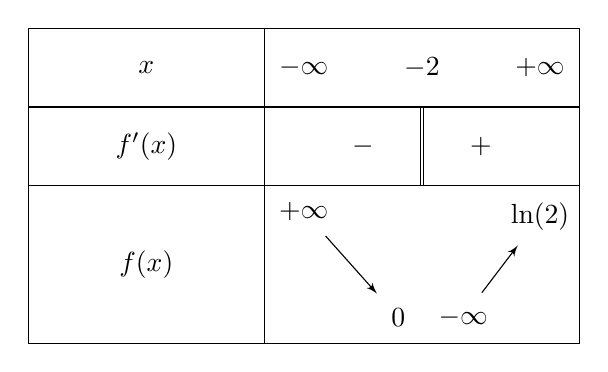
\begin{tikzpicture}
   \tkzTabInit[lgt=3,espcl=1.5]
     {$x$ / 1 , $f'(x)$ / 1, $f(x)$ / 2}
     {$-\infty$, $-2$, $+\infty$}
   \tkzTabLine
     { , -, d , + , }  % 'd' pour descendre le trait à x = -2
   \tkzTabVar
     {+/$+\infty$, -V-/ $0$ / $-\infty$, +/$\ln(2)$}  % Correction ici
\end{tikzpicture}
\end{center}

\end{enumerate}
\item
\begin{enumerate}
    \item Déterminons les intersections de $A$ et $B$ de $\mathcal{C}_{f}$ avec $(Ox)$ et $(Oy)$ respectivement.
    
    \underline{ \textbf{ ($\mathcal{C}_{f}$) avec $(Ox)$ } }

    Pour ce faire résolvons de $f(x)=0$
\[
\begin{aligned}
    \begin{cases}
    \sqrt{x^2 + 2x} = 0 \\
    \ln\left( \frac{2x+4}{x+3} \right) = 0
\end{cases} &\implies
\begin{cases}
    x^2 + 2x = 0 \\
    \frac{2x+4}{x+3} = 1
\end{cases}\\
 &\implies
\begin{cases}
    x= 0 \text{ ou } x = -2 \text{ si } x \leq -2\\
    x=-1 \text{ si } x > -2
\end{cases}\\
\end{aligned}
\]

\( A_{-1} \begin{pmatrix} -2 \\ 0 \end{pmatrix} \text{ et } A_{-2} \begin{pmatrix} -1 \\ 0 \end{pmatrix} \) 

\underline{ \textbf{ ( \( \mathcal{C}_{f} \) ) avec \( (Oy) \) } }

    Pour ce faire calculons de $f(0)$

    \( f(x) = \ln\left( \frac{2x+4}{x+3} \right) \)
    
    \( f(0) = \ln\left( \frac{2 \times 0+4}{0+3} \right) \)

donc \( f(0) = \ln\left( \frac{4}{3} \right) \)

$ B \begin{pmatrix} 0 \\ \ln\left( \frac{4}{3} \right) \end{pmatrix} $

\item Equation de la tangente \( (T) \) à \( (\mathcal{C}_{f}) \) en \( A\begin{pmatrix} -1 \\ 0 \end{pmatrix} \)

\( (T) \): \( y = f'(-1) (x+1)  + f(-1) \)

Or \( f'(-1) = \frac{2}{(-1+3)(-2+4)} \) donc \( f'(-1) = \frac{1}{2} \)

et \( f(-1) = 0 \)

\( (T) \): \( y = \frac{1}{2} \times (x+1) \)

\( (T) \): \( y = \frac{1}{2}x+\frac{1}{2} \)
\item La courbe 
\begin{center}
\begin{figure}[H]% Forcer l'image à cet endroit
\centering
\includegraphics[width=0.8\textwidth]{Devoir1Curve.png}
\caption{Courbe de (Cf)}
\label{fig:monimage}
\end{figure}
\href{https://www.geogebra.org/classic/ud3zvetx}{Clique ici pour voir la courbe sur géogébra}\\
\end{center}
\end{enumerate}

\end{enumerate}

\subsection*{Partie C}

Soit \( h \) la restriction de \( f \) à \( I = ]-\infty; -2 [ \)

\begin{enumerate}
    \item Montrer que \( h \) est une bijection de \( I \) vers un intervalle \( I \) à préciser.

    \( h \) est continue et strictement décroissante sur \( I \) donc réalise une bijection de \( I \) vers \( f(I) = J \)

    avec \( J = [ 0; +\infty [ \)

    \item 
    \begin{enumerate}
        \item \( h^{-1} \) est-elle dérivable sur J ?
    
    Comme \( h \) étant dérivable sur \( I \) et que  \( \forall x\in I, h'(x) \neq 0 \) donc \( h^{-1} \) est dérivable sur \( J \).

    Ainsi, \( h^{-1} \) est bien dérivable sur \( J \).

\begin{align*}
h:]-\infty ; -2[&\rightarrow ]0; +\infty [\\
x&\mapsto h(x)
\end{align*}
\begin{align*}
h^{-1}:]0; +\infty [&\rightarrow ]-\infty ; -2[\\
y&\mapsto h^{-1}(y)
\end{align*}

    \item Dressons le tableau de \( h^{-1} \)

    \begin{center}
        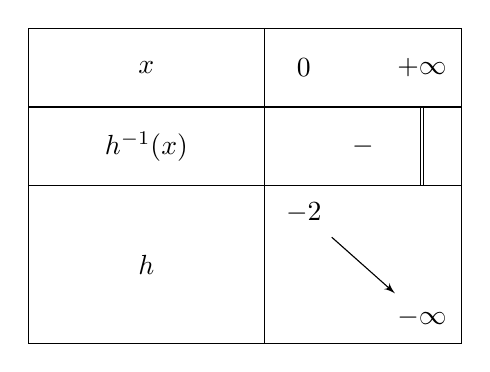
\begin{tikzpicture}
        \tkzTabInit[lgt=3,espcl=1.5]
        {$x$ / 1 , $h^{-1}(x)$ / 1, $h$ / 2}
        {$0$, $+\infty$}
        \tkzTabLine
        { , -,d}  % 'd' pour descendre le trait à x = -2
        \tkzTabVar
        {+/$-2$, -/$-\infty$}  % Correction ici
        \end{tikzpicture}
    \end{center}
    Calculons \( h(-3) \textbf{ et } (h^{-1})'( \sqrt{3} )  \)

    \( h(x) = \sqrt{x^{2}+2x} \)

    \underline{\textbf{Pour}  \( h(-3)  \) } : 

\(
    \begin{aligned}
        h(-3) &= \sqrt{(-3)^{2}+2(-3)}\\
              &= \sqrt{9 - 6}\\
              &= \sqrt{3}
    \end{aligned}
\)

\( \text{Donc } \boxed{ h(-3)=\sqrt{3} } \)

    \underline{\textbf{Pour} \( (h^{-1})'( \sqrt{3} )  \) }:
\[\text{On a : }  (h^{-1})'(y) = \frac{1}{h'(h^{-1}(y))} \text{donc } (h^{-1})'(\sqrt{3}) = \frac{1}{h'(h^{-1}(\sqrt{3}))}\]

Calcul de \( h^{-1}(\sqrt{3}) \):

On sait que \( h(-3) = \sqrt{3} \), donc \( h^{-1}(\sqrt{3}) = -3\)

Donc \( (h^{-1})'(\sqrt{3}) = \frac{1}{h'(h^{-1}(\sqrt{3}))}\) devient \( (h^{-1})'(\sqrt{3}) = \frac{1}{h'(-3)}\)

Calcul de \( h'(-3) \):

\(
\begin{aligned}
   h'(-3) &= \frac{-3+1}{\sqrt{(-3)^2 + 2(-3)}}\\
          &= \frac{-2}{\sqrt{9 - 6}}\\
          &= \frac{-2}{\sqrt{3}}\\
          &= -\frac{2\sqrt{3}}{3}
\end{aligned}
\)

Calcul de \( (h^{-1})'(\sqrt{3}) \)

\(
\begin{aligned}
(h^{-1})'(\sqrt{3}) &= \frac{1}{h'(-3)}
                    &= \frac{1}{-\frac{2\sqrt{3}}{3}}
                    &= -\frac{3}{2\sqrt{3}}
                    &= -\frac{\sqrt{3}}{2}
\end{aligned}
\)

\[
\boxed{(h^{-1})'(\sqrt{3}) = -\frac{\sqrt{3}}{2}}
\]
\item Explicitons \( (h^{-1})'(x) \)

\begin{align*}
h^{-1}:]0; +\infty [&\rightarrow ]-\infty ; -2[\\
x&\mapsto h^{-1}(x)
\end{align*}


\begin{align*}
    h(x) &= y\\
\sqrt{x^2 + 2x} &= y\\
    x^2 + 2x &= y^2\\
    x^2 + 2x - y^2 &= 0
\end{align*}
Résolvons l'équation \( x^2 + 2x - y^2 = 0 \) en \(x\)

\(
\begin{aligned}
    \Delta &= 2^{2}-4(1)(-y^2)\\
           &=4+4y^2
\end{aligned}
\)

\( x = \frac{-2 - \sqrt{4 + 4y^2}}{2} \) ou \( x = \frac{-2 + \sqrt{4 + 4y^2}}{2} \)

Puisque \( \forall x \in ]0; +\infty [ \), \( h^{-1}(x) < 0 \), nous devons choisir la solution qui respecte cette condition.

On en déduit que :

\[
\tcbhighmath[boxrule=1pt, colback=yellow!5!white, colframe=black]{ h^{-1}(x) = -1 - \sqrt{1 + x^2} }
\]
    \end{enumerate}
\end{enumerate}
\end{document}
